\documentclass[border=15pt, multi, tikz]{standalone}
\usepackage{import}
\subimport{./layers/}{init}
\usetikzlibrary{positioning}
\usetikzlibrary{3d} %for including external image 
\def\ConvColor{rgb:yellow,5;red,2.5;white,5}
\def\ConvReluColor{rgb:yellow,5;red,5;white,5}
\def\PoolColor{rgb:red,1;black,0.3}
\def\DcnvColor{rgb:blue,5;green,2.5;white,1}
\def\SoftmaxColor{rgb:magenta,5;black,7}
\def\SumColor{rgb:blue,5;green,15}
\def\BallColor{rgb:blue,5;green,2.5;white,5}
\def\verdognolo{rgb:green,5;white,2}

\begin{document}

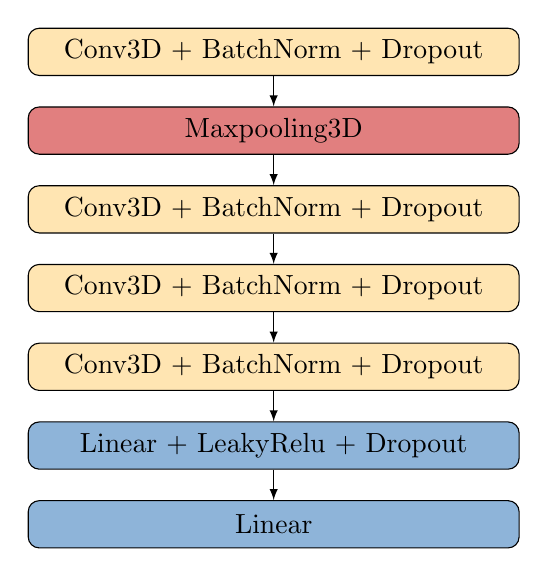
\begin{tikzpicture}
\tikzstyle{connection}=[ultra thick,every node/.style={sloped,allow upside down},draw=\edgecolor,]
\tikzstyle{pool} = [rectangle, draw, fill=\PoolColor, text width=6cm, text centered, rounded corners, minimum height=0.6cm, fill opacity=0.5, text opacity=1]
 \tikzstyle{conv} = [rectangle, draw, fill=\ConvColor, text width=6cm, text centered, rounded corners, minimum height=0.6cm, fill opacity=0.5, text opacity=1]
 \tikzstyle{lin} = [rectangle, draw, fill=\DcnvColor, text width=6cm, text centered, rounded corners, minimum height=0.6cm, fill opacity=0.5, text opacity=1]
\tikzstyle{connector} = [draw, -latex]
\tikzstyle{line} = [line, -latex]

  \tikzstyle{decision} = [rectangle, minimum width=0cm, minimum height=1cm, text centered, draw=black, opacity=0]

\node  [conv] at (0,0) (c1) {Conv3D + BatchNorm + Dropout};
\node [pool] at (0,-1) (p1) {Maxpooling3D };
\node [conv] at (0,-2) (c2) {Conv3D + BatchNorm + Dropout};
\node [conv] at (0,-3) (c3) {Conv3D + BatchNorm + Dropout};
\node [conv] at (0,-4) (c4) {Conv3D + BatchNorm + Dropout};
\node [lin] at (0,-5) (l1) {Linear + LeakyRelu + Dropout};
\node [lin] at (0,-6) (l2) {Linear};


\path [connector] (c1) -- (p1);
\path [connector] (p1) -- (c2);
\path [connector] (c2) -- (c3);
\path [connector] (c3) -- (c4);
\path [connector] (c4) -- (l1);
\path [connector] (l1) -- (l2);



\end{tikzpicture}



\end{document}\grid